%%%%%%%%%%%%%%%% Preamble begins %%%%%%%%%%%%%%%%
\documentclass[aspectratio=169,mathserif,10pt]{beamer}
\beamertemplatenavigationsymbolsempty
\usepackage[utf8]{inputenc}
\usepackage{graphicx} % needed to insert figures
\usepackage{tikz} % needed to draw graphical elements
\usepackage[many]{tcolorbox} % the option many is needed for fancy, shaded boxes
\tcbuselibrary{skins} % needed for the dashed box
\usepackage{media9} % needed to embed videos in pdf
\usepackage{amsmath} % needed to type beautiful math

\usepackage{soul} % needed to strike out some text

% to be able to use path in tikz figures
\usetikzlibrary{calc,patterns,decorations.pathmorphing,decorations.markings}
% to be able to compute intersections in tikz figures
\usetikzlibrary{intersections}
% to be able to do other decorations in tikz figures
\usetikzlibrary{shapes.misc}
\usetikzlibrary{decorations.pathreplacing}

% to be able to do other fancy stuff in tikz figures
\usetikzlibrary{arrows,decorations.markings}
\usetikzlibrary{arrows.meta}
\newcommand{\tikzAngleOfLine}{\tikz@AngleOfLine}

% for tikz special symbols
\usetikzlibrary{shapes.misc}
\usetikzlibrary{patterns,decorations.pathreplacing}
\tikzset{cross/.style={cross out, draw=black, minimum size=2*(#1-\pgflinewidth), inner sep=0pt, outer sep=0pt},
%default radius will be 1pt.
cross/.default={1pt}}

%%% theme
\usetheme[compress]{Berlin}

%% Some customization here

% this sets a footnote rule, of a desired color and thickness
\renewcommand\footnoterule{{\color{black}\rule{\paperwidth}{.5pt}}}

% here we define the footline field, with 3 subfields
\setbeamertemplate{footline}{

% first, let's place the footnote rule we defined above
\footnoterule

% then, let's define the footline field with 3 subfields, i.e., beamercolorboxes
\hbox{%
    \begin{beamercolorbox}[wd=0.3\framewidth,ht=2.25ex,dp=1ex,left]{footlinecolor}
        \usebeamerfont{author in head/foot}\hspace*{1em}{\insertshortauthor}
    \end{beamercolorbox}%
    \begin{beamercolorbox}[wd=0.3\framewidth,ht=2.25ex,dp=1ex,center]{footlinecolor}
        \usebeamerfont{title in head/foot}{\insertshorttitle}
    \end{beamercolorbox}%
    \begin{beamercolorbox}[wd=0.3\framewidth,ht=2.25ex,dp=1ex,right]{footlinecolor}
        \usebeamerfont{institute in head/foot}{\insertshortinstitute}
    \end{beamercolorbox}%
    \begin{beamercolorbox}[wd=0.03\framewidth,ht=2.25ex,dp=1ex,right]{footlinecolor}
        \hspace*{12em}
        \insertframenumber\,/\,\inserttotalframenumber 
    \end{beamercolorbox}%
    }
}

% I don't like squared bullet points, so let's change them to round bullets
\setbeamertemplate{itemize items}[ball] \setbeamertemplate{enumerate
items}[ball]

% A CU color scheme (thanks to Gary Nave!) complete with logo
% define a custom color in cmyk scale (percentage)
\definecolor{CUgold}{cmyk}{0,0.1,0.48,0.22}
% define a custom color in rgb scale (percentage)
\definecolor{CUdarkgray}{rgb}{0.74,0.74,0.74}
% define a custom color in RGB scale ([0,255])
\definecolor{CUlightgray}{RGB}{233,233,233}
% assign colors to different structures of the frame
\setbeamercolor*{structure}{bg=CUgold,fg=black}
\setbeamercolor*{palette primary}{use=structure,fg=black,bg=CUlightgray}
\setbeamercolor*{palette secondary}{use=structure,fg=black,bg=structure.bg}
\setbeamercolor*{palette tertiary}{use=structure,fg=white,bg=structure.fg}
\logo{
\includegraphics[width=1.25in,trim={0in 0in 0in 0in},clip]{Images/CUBoulderLogo.png}}

% This command allows you to make a slide without the logo
% Ex: {\nologo \begin{frame}... \end{frame} }
\newcommand{\nologo}{\setbeamertemplate{logo}{}}

% This is a shortcut I use to create a new slide
\newcommand{\newslide}[2]
{\begin{frame}{#1}
\begin{center}
{#2}
\end{center}
\end{frame}}

% These commands allow for backup slides without affecting numbering
\newcommand{\backupbegin}{
	\newcounter{framenumberappendix}
	\setcounter{framenumberappendix}{\value{framenumber}}
}
\newcommand{\backupend}{
	\addtocounter{framenumberappendix}{-\value{framenumber}}
	\addtocounter{framenumber}{\value{framenumberappendix}}
}

%% end of customization

%% general info: title, author, institution, date
\title[short title]{Long title}
%\title[Intro on \LaTeX]{Postdoc Tutorial: Intro on \LaTeX}
\author[short author]{Long author}
%\author[Valeria Barra]{Valeria Barra}
\institute[Short institute]{Full institute: \\
University of Colorado Boulder}
\date[Short date]{
    Long date \\ 
    Name of conference \\ 
    Month dd, yyyy\\
    % include a picture to ackowledge sponsors, if you like
    \centering
    \vspace{.7cm}
    \includegraphics[scale=0.2]{Images/DOELogo.jpg}
    \hspace{2cm}
    \includegraphics[scale=0.22]{Images/NSFLogo}
}

%%%%%%%%%%%%%%%% Preamble ends %%%%%%%%%%%%%%%%

%---------------------------------------------%

%%%%%%%%%%%% Actual document begins %%%%%%%%%%%%

%% Begin document
\begin{document}
	
{\nologo 
    {\setbeamertemplate{footline}{}
        \begin{frame}[noframenumbering]
            \maketitle
        \end{frame}
    }
}

%% Introduction
\section[Intro]{Introduction}

\begin{frame}
\frametitle{Our first slide (a.k.a. frame)}
    
Hello world!

\pause
\Large{Let's type some large text.}

\pause
\LARGE{Let's type some very large text.}

\pause 
or some \textcolor{red}{colored text}, some \textbf{bold text}, some \emph{italic text}, some \underline{underlined text} and some \st{struck-out text}.
    
\end{frame}

\newslide{Automatically generated outline}{
    % this will automatically generate the table of contents, based on your declard sections and subsections
    \tableofcontents
}

% What if I don't like the automatically generated table of contents? Let's create an itemized list!
\newslide{My very personal outline}{

\begin{enumerate}
    \item Introduction
    \item A great section we're going to talk about
    \item Yet another great section we're going to talk about
    \begin{itemize}
        \item Hey, this section requires some in-depth thought
        \item So here I have an itemized list within a list
    \end{itemize}
    \item Conclusions
\end{enumerate}

}

%% Section 1
\section[Sec. 1]{Section 1}
\subsection[Subsection 1.1]{Subsection 1.1}

\begin{frame}
\frametitle{Another section, another slide}

\end{frame}


%% Section 2
\section[Sec. 2]{Section 2}
% if you need to remind your audience where you were at
\frame{\tableofcontents[currentsection]}

\newslide{A slide with a movie!}{
% let's insert a video
\includemedia[
    width=8.5cm,height=4.5cm,
    activate= pageopen,
    deactivate=onclick,
    addresource=./Videos/NSTAdvectionCori061.swf,
    flashvars={
        source=./Videos/NSTAdvectionCori061.swf
       &autoPlay=true
    }
]{}{./Videos/NSTAdvectionCori061.swf}


}

%% Math Section
\section[Math Section]{Math Section}

\newslide{Let's type some math}{

To use inline math-mode, you need to enclose the symbols in \$ \$, for instance $x = \frac{-b \pm \sqrt{b^2-4ac}}{2a}$.

To use display math-mode, i.e., for better spacing and aesthetics use \textbackslash[ \textbackslash], for instance 

\[x = \frac{-b \pm \sqrt{b^2-4ac}}{2a}\]

or, with the double \$\$ \$\$ symbol 

$$
x = \frac{-b \pm \sqrt{b^2-4ac}}{2a}
$$
}

\newslide{Some math: align vs align*}{

\vspace{-.5cm}

\begin{minipage}{0.48\textwidth}
    \begin{align}
    I &= \scriptstyle{\int_{-\infty}^{\infty}\frac{1}{\sqrt{2\pi}}\mbox{e}^{-x^2/2}dx}\\
      &= \scriptstyle{\sqrt{\int_{-\infty}^{\infty}\frac{1}{\sqrt{2\pi}}
    \mbox{e}^{-x^2/2}dx\int_{-\infty}^{\infty}
    \frac{1}{\sqrt{2\pi}}\mbox{e}^{-y^2/2}dy}}\nonumber\\
      &= \scriptstyle{\sqrt{\frac{1}{2\pi}\int_0^{\infty}
    \int_0^{2\pi}r\mbox{e}^{-r^2/2}drd\theta}}\\
      &= \scriptstyle{1}
    \end{align}
\end{minipage}

\begin{minipage}{0.48\textwidth}
    \begin{align*}
    I &= \scriptstyle{\int_{-\infty}^{\infty}\frac{1}{\sqrt{2\pi}}\mbox{e}^{-x^2/2}dx}\\
      &= \scriptstyle{\sqrt{\int_{-\infty}^{\infty} \frac{1}{\sqrt{2\pi}}
    \mbox{e}^{-x^2/2}dx\int_{-\infty}^{\infty}
    \frac{1}{\sqrt{2\pi}}\mbox{e}^{-y^2/2}dy}}\\
      &= \scriptstyle{\sqrt{\frac{1}{2\pi}\int_0^{\infty}
    \int_0^{2\pi}r\mbox{e}^{-r^2/2}drd\theta}}\\
      &= \scriptstyle{1}
    \end{align*}
\end{minipage}

}

\begin{frame}{Some more math}
\vspace{-.3cm}

A system of equations with same number:

{\small
    \begin{subequations}\label{NSEqns}
        \begin{align}
        \frac{\partial \rho}{\partial t} + \nabla \cdot \boldsymbol{U} &= 0 \, ,\\
        \frac{\partial \boldsymbol{U}}{\partial t} + \nabla \cdot \left( \frac{\boldsymbol{U} \otimes \boldsymbol{U}}{\rho} + P \mathbf{I}_3 \right) + \rho g \boldsymbol{k} &= \nabla \cdot \boldsymbol{\sigma} \, ,\\
        \frac{\partial E}{\partial t} + \nabla \cdot \left( \frac{(E + P)\boldsymbol{U}}{\rho} \right) &= \nabla \cdot \left(  \boldsymbol{u}  \cdot \boldsymbol{\sigma}  + k \nabla T\right)\, ,
        \end{align}
    \end{subequations}
}


A very long expression that corresponds to one equation only

\begin{minipage}{0.48\textwidth}
\begin{align}
\sum_{i=0}^{N} A =& A + A + A + \ldots + A + \nonumber \\
                  & A + A + A + \ldots + A \,.
\end{align}
\end{minipage}

\end{frame}

\newslide{Arrays}{

\begin{align*}
    \begin{array}{r}
        P \\
        \mu \\
        g 
    \end{array}
    \begin{array}{l}
        \leftarrow\textrm{ pressure}\\
        \leftarrow\textrm{ dynamic viscosity}\\
        \leftarrow\textrm{ gravitational acceleration}
    \end{array}
\end{align*}

A matrix: 

\begin{align}
    \begin{array}{rl}
        \mathbf{A} = &
        \left[
        \begin{array}{c c c}
            a_{11} & a_{12} & a_{13} \\
            a_{21} & a_{22} & a_{23} \\
            a_{31} & a_{32} & a_{33}
        \end{array}
        \right]
    \end{array} \,
\end{align}

}

%% Boxes Section
\section[Boxes]{Boxes}

\newslide{Boxes}{

\begin{columns}

\column{.49\linewidth}
    \begin{tcolorbox}[halign=left,width=4cm,colback=red!5!white,colframe=red!75!black,title=A nice box]
        Indeed.
    \end{tcolorbox}
    
    \begin{tcolorbox}[width=4cm,leftrule=3mm,colback=red!5!white,colframe=red!75!black]
        A box with a left rule.
    \end{tcolorbox}
    
    \begin{tcolorbox}[enhanced,frame empty,interior empty,width=4cm,borderline={0.5mm}{0mm}{black!50!white,dashed}]
        A dashed box
    \end{tcolorbox}
   

\column{.49\linewidth}
    \begin{tcolorbox}[width=4cm,colback=blue!5!white,colframe=blue!75!black,arc=0mm]
        This is a box with no rounded corners.
    \end{tcolorbox}
    
    \begin{tcolorbox}[width=4cm,colback=blue!5!white,colframe=blue!75!black,arc=3mm]
        This is a a box with rounded corners.
    \end{tcolorbox}
    
    \begin{tcolorbox}[width=3cm,
        colback=green!5!white,
        colframe=green!75!black,
        halign=center,valign=center,
        square,circular arc]
        This is also a box!
    \end{tcolorbox}

\end{columns}


}

%% Extra Section
\section[Extra]{Extra}

%% some backup slides
\backupbegin

\begin{frame}
\frametitle{Example of a backup slide}

Note the frame number!

\end{frame}


\begin{frame}
\frametitle{Let's do some graphics!}

We need the \textcolor{red}{Tikz} package loaded in the preamble.

Let's draw a cross.


\begin{tikzpicture}
    \draw (0,0) node[cross=3.5pt,red]{};
\end{tikzpicture}

Let's draw a filled circle.


\begin{tikzpicture}
    \fill[blue] (0,0) circle(3.5pt);
\end{tikzpicture}

 Let's draw a horizontal segment.

\begin{tikzpicture}
    \draw (0,0) -- (2,0);
\end{tikzpicture}

Let's draw a vertical annotated segment.

\begin{tikzpicture}
    \draw (1,1)node[anchor=south]{A} -- (1,0) node[anchor=north]{B};
\end{tikzpicture}

\end{frame}

\begin{frame}
\frametitle{Exercise}

Draw a square and annotate its vertices.

\end{frame}


\begin{frame}{A more complicated example}

\resizebox{0.75\textwidth}{!}{
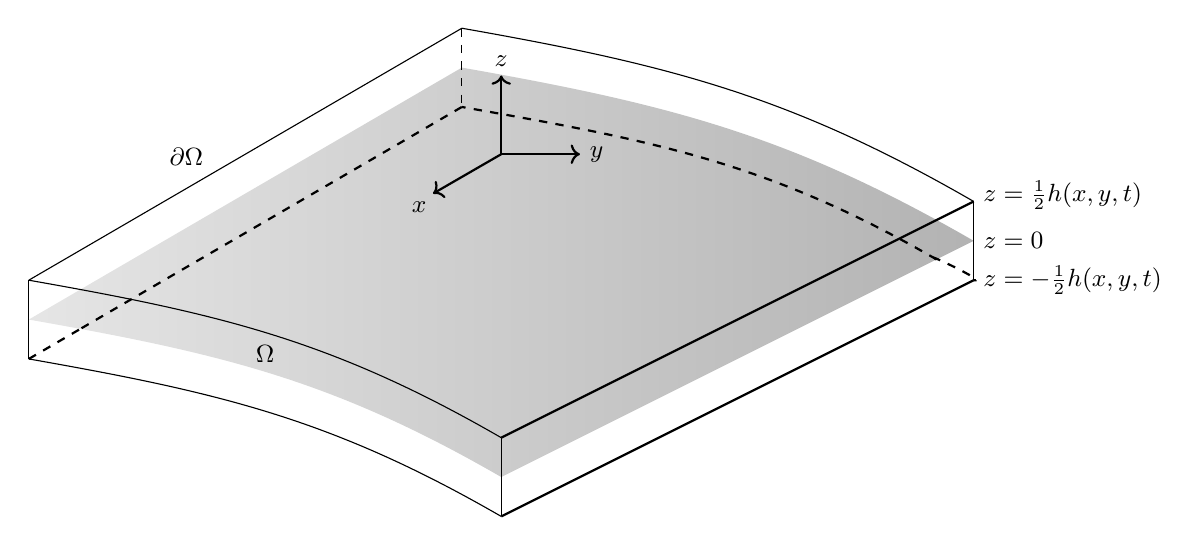
\begin{tikzpicture}
    \tikzstyle{ground}=[fill,pattern=north east lines,draw=none,minimum width=0.3,minimum height=0.6]
    \tikzstyle{every node}=[font=\small]
    
    % only path of the shaded mid-surface
    % mid-border 1
    \path[name path=border-mid1] (0,-0.5) to[out=-10,in=150] (6,-2.5);
    % mid-border 2
    \path[name path=border-mid2] (6,-2.5) -- (12,0.5);
    % mid-border 3
    \path[name path=border-mid3] (12,0.5) to[out=150,in=-10] (5.5,2.7);
    % mid-border 4
    \path[name path=border-mid4] (5.5,2.7) -- (0,-0.5);
    
    % draw the shaded mid-surface
    \shade[left color=gray!20,right color=gray!60]
      (0,-0.5) to[out=-10,in=150] (6,-2.5) --
      (12,0.5) to[out=150,in=-10] (5.5,2.7) -- cycle;
    
    % axis
    \draw[thick,->] (6,1.6) -- +(0,1)  node[yshift=5pt] {$z$};
    \draw[thick,->] (6,1.6) -- +(210:1) node[yshift=-5pt,xshift=-5pt] {$x$};
    \draw[thick,->] (6,1.6) -- +(1,0) node[xshift=6pt] {$y$};
    % labels for surfaces
    \draw (12,1.08) node[anchor=west]{$z= \frac{1}{2}h(x,y,t)$};
    \draw (12,0.5) node[anchor=west]{$z=0$};
    \draw (12,0) node[anchor=west]{$z=- \frac{1}{2}h(x,y,t)$};
    \draw (3,-0.7) node[anchor=north]{$\Omega$};
    \draw (2,1.8) node[anchor=north]{$\partial\Omega$};
    
    % border of the upper surface border 1
    \path[draw,name path=border-up1] (0,0) to[out=-10,in=150] (6,-2);
    % border of the upper surface border 2
    \draw[draw,thick,name path=border-up2] (6,-2) -- (12,1);
    % border of the upper surface border 3
    \path[draw,name path=border-up3] (12,1) to[out=150,in=-10] (5.5,3.2);
    % border of the upper surface border 4
    \path[draw,name path=border-up4] (5.5,3.2) -- (0,0);
    
    % border of the lower surface border 1
    \path[draw,name path=border-bottom1] (0,-1) to[out=-10,in=150] (6,-3);
    % border of the lower surface border 2
    \draw[draw,thick,name path= border-bottom2] (6,-3) -- (12,0);
    % border of the lower surface border 3
    \path[name path=border-bottom3] (12,0) to[out=150,in=-10] (5.5,2.2);
    % border of the lower surface border 4
    \path[name path=border-bottom4] (5.5,2.2) -- (0,-1);
    
    % intersection points
    \path[name intersections={of=border-mid1 and border-bottom4,by={a}}];
    \path[name intersections={of=border-mid2 and border-bottom3,by={b}}];
    
    % draw dashed and solid lines for hidden borders
    \draw[draw,thick,dashed,name path=border-bottom-dashed4] (5.5,2.2) -- (a);
    \draw[draw,thick,dashed,name path=border-bottom-solid4] (0,-1) -- (a);
    \draw[draw,thick,dashed,name path=border-bottom-dashed3] (b) to[out=150,in=-10] (5.5,2.2) ;
    \draw[draw,thick,dashed,name path=border-bottom-solid3] (b) to[out=150,in=-10] (12,0) ;
    
    % draw vertical segments
    \path[draw, name path=border-v1] (0,0) -- (0,-1);
    \path[draw, name path=border-v2] (6,-2) -- (6,-3);
    \path[draw, name path=border-v3] (12,1) -- (12,0);
    \path[draw, dashed, name path=border-v4] (5.5,3.2) -- (5.5,2.2);
    
    % \end{axis}
\end{tikzpicture}
}

\end{frame}

\newslide{Thanks}{

\begin{tcolorbox}[width=5cm,halign=center,enhanced,colback=white,colframe=black!50!white,boxrule=1pt,
  arc=3pt,outer arc=3pt,drop lifted shadow=]
  
\LARGE{Thank you!}

\end{tcolorbox}

}

\backupend



\end{document}
%%%%%%%%%%%% Actual document ends %%%%%%%%%%%%
